\documentclass[12pt]{article}
\usepackage[utf8]{inputenc}
\usepackage[T1]{fontenc}
\usepackage[english]{babel}
\usepackage{ifpdf,newtxtext,newtxmath} 
\usepackage{array,graphicx,dcolumn,multirow,hevea,abstract,hanging,fancyhdr,float}
% change next 3 lines each issue
\newcommand{\jref}{http://journal.sjdm.org/vol16.1.html}
\newcommand{\jhead}{Judgment and Decision Making, Vol.~16, No.~1}
\newcommand{\jdate}{January 2021}
\topmargin=-.3in \oddsidemargin=.3in \evensidemargin=.3in \textheight=9in \textwidth=6in
%\pagestyle{fancy} 
%\fancyhead[L]{\protect\small \href{\jref}{\jhead}, \jdate}
%\fancyhead[R]{\protect\small SHORT TITLE} % replace with running head
%\fancyhead[L]{}
%\fancyhead[R]{} % replace with running head
%\fancypagestyle{firstpage}{%
%\lhead{\protect\small \href{\jref}{\jhead}, \jdate}
%\lhead{}
%\rhead{}
%}
\usepackage[labelfont=sc,textfont=sf]{caption}
\usepackage[hyperfootnotes=false,breaklinks=true]{hyperref} % was dvipdfmx
% \usepackage[hyperfootnotes=false,breaklinks=true,linkbordercolor={1 1 1},citebordercolor={1 1 1}]{hyperref}
% \usepackage{natbib} % must come afer hyperfootnotes, use 2nd version for bibtex
% \setlength{\bibsep}{0pt}
\urlstyle{rm}
\usepackage[hyphenbreaks]{breakurl}
% DO NOT USE ADDITIONAL PACKAGES unless you make sure they work with Hevea.
% You may define new commands, but these may cause other troubles, so try to avoid it.

% FOR BIBTEX USERS (Bibtex is not recommended, but we can use it):
% \usepackage{natbib} % must come afer hypperref
% in references: \bibliographystyle{apalike3} \setlength{\bibsep}{0pt} \bibliography{WHATEVER}
% download http://journal.sjdm.org/apalike3.bst
\usepackage{booktabs} % \toprule \midrule \bottomrule \cmidrule(lr){a-b}
% define centered and ragged columns:
\newcolumntype{L}[1]{>{\raggedright\arraybackslash }p{#1}} % can use m{}
\newcolumntype{C}[1]{>{\centering\arraybackslash }p{#1}}
\newcolumntype{R}[1]{>{\raggedleft\arraybackslash }p{#1}}
\newcolumntype{d}[1]{D{.}{.}{#1}} % d{3.2} for 3 places on l, 2 on r
\newcommand{\mc}{\multicolumn}
\setlength\tabcolsep{1mm}
\setlength\columnsep{5mm}
\setlength\abovecaptionskip{1ex}
\setlength\belowcaptionskip{.5ex}
\setlength\belowbottomsep{.3ex}
\setlength\lightrulewidth{.04em}
\renewcommand\arraystretch{1.2}
\renewcommand{\topfraction}{1}
\renewcommand{\textfraction}{0}
\renewcommand{\floatpagefraction}{.9}
% \renewcommand{\baselinestretch}{1.00} \large\normalsize % for fixing spaces
\widowpenalty=1000
\clubpenalty=1000
\setlength{\parskip}{0ex}
\let\tempone\itemize
\let\temptwo\enditemize
\let\tempthree\enumerate
\let\tempfour\endenumerate
\renewenvironment{itemize}{\tempone\setlength{\itemsep}{0pt}}{\temptwo}
\renewenvironment{enumerate}{\tempthree\setlength{\itemsep}{0pt}}{\tempfour}

%%%%%%%%%%%%%%%%%%%%%%%%%%%%%%%%%%%%%%%%%%%%%%%%%%%%%%%%%%%%%%%%%%%%%
\setcounter{page}{1} % start with first page

\title{Measuring the effect of COVID-19 lockdowns on air quality and the impact on child health using machine learning}

\author{
Jonathan Baron\thanks{Department of Psychology, University of
  Pennsylvania. Email: baron@upenn.edu.}\;\,\thanks{Some other address.}
\and 
  Some O. Person\thanks{Yet another place.} 
\and
  Y. Another Author\footnotemark[2] % indicates same as 2nd thanks
}

\date{} % leave empty
\begin{document} % goes here

\begin{htmlonly}
\href{\jref}{\jhead}, \jdate, pp.\
\end{htmlonly}

\maketitle
%\thispagestyle{firstpage}

\begin{abstract}

The abstract is a brief (usually one paragraph) summary
of the whole paper, including the problem, the method for solving
it (when not obvious), the results, and the conclusions suggested
or drawn.  Do not write the abstract as a hasty
afterthought. Look at it as a real exercise in cramming the most
information in one paragraph.  The reader should not have to read
any of the rest of the paper in order to understand the abstract
fully.  Many readers will read only the abstract.  Other readers
will use it to decide what to look for in the paper, or to decide
whether to read the whole thing.  Remember 
\href{http://en.wikipedia.org/wiki/The_Elements_of_Style}{Strunk \&
  White's} admonition, ``Omit needless words.''

\smallskip
\noindent
Keywords: journal, template, latex
\end{abstract}

{\renewcommand{\thefootnote}{}
\footnotetext{ % note blank lines above and below acknowledgment

  Portions of this template are shamelessly stolen from other
  documents lying around on the author's computer. He is grateful to
  Lenovo, Inc.

Copyright: \copyright\ 2021.
The authors license this article under the terms of the
\href{http://creativecommons.org/licenses/by/3.0/}{Creative Commons
  Attribution 3.0 License.}
}}

\saythanks

\setlength{\baselineskip}{16pt plus.2pt}

\section{Introduction}\label{sec:intro}
UNICEF and Solve for Good have partnered together to analyze various aspects of changes in air pollution — especially related to COVID-19 and with the long-term goal to build a platform for air pollution monitoring with a strong emphasis on UNICEF’s operations, with focus on
\begin{itemize}
    \item Developing a model to measure children’s exposure to air pollutant PM2.5, which exceeds the WHO Standard in the present COVID Scenario.
    \item Understanding the air quality level around the globe with the target of attaining a fine-grained estimation from the combination of Ground value measurement from openly available ground sensor measurements and Remote Sensing
    \item Enabling Citizen Scientists to delve deeper and get involved in Air Quality Measurement globally.
\end{itemize} 
%
Specifically, we aim to (a) model the impact of COVID19 lockdowns on air quality and (b) test whether this has led to an improvement in children’s health. Following the footsteps of existing works like \citet{Borneman,Mahato}, we hypothesize to find evidence of the positive effects of air quality resulting from the large-scale modal shift to low emissions vehicles post lockdown develop an exploratory visualization platform for local program managers. The platform will provide functions to manage, analyze, and visualize changes in air pollution data at different locations preferably, in countries and cities where UNICEF operates with interests in air pollution monitoring for children’s health.

Globally, 93\% of children live in environments where air pollution levels exceed WHO guidelines. There is a strong link between human health and exposure to high levels of air pollution. Long-term exposure to fine particulate matter with a diameter less than 2.5$\mu$m (PM2.5) are estimated to cause ~8 million excess deaths annually. Simultaneously, nitrogen dioxide (NO$_2$) results in 4 million new pediatric asthma cases annually \cite{Venter}. The impact of air pollution is felt more acutely by the young, with one in every four deaths of children under 5 years is directly or indirectly related to environmental risks \cite{who}.

However, the child population’s distribution does not correspond well to the global distribution of air quality sensors. Illustrating these distributions are panel (a) of Figure~\ref{fig:maps} showing the locations of air quality sensors and panel (b) the global concentration of child populations. Therefore using only the locations of ground-source air quality sensors to infer the effects of exposure to high levels of air pollution on global child populations is difficult, particularly in high populous locations such as Western Africa and the Great Rift Valley.

\begin{figure*}
    \centering
    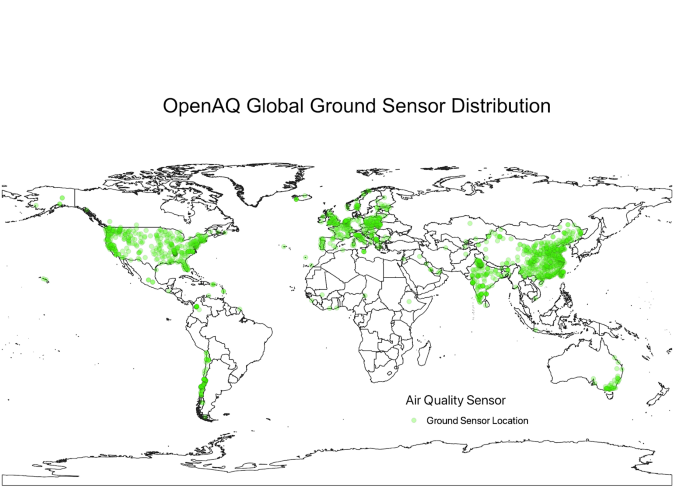
\includegraphics[width=.49\textwidth]{sensormap.png}
    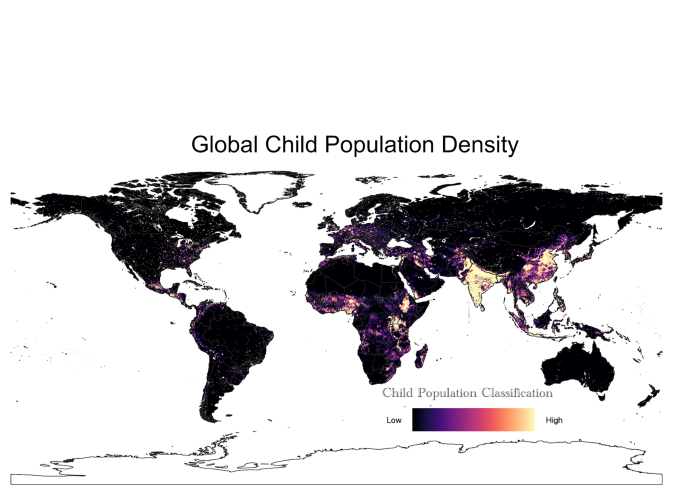
\includegraphics[width=.49\textwidth]{childmap.png}
    \caption{Global distribution of (a) air quality sensors, and (b) Child Population, data source: Silent Suffocation in Africa, UNICEF-2019.}
    \label{fig:maps}
\end{figure*}

During the Covid-19 lockdowns, fossil fuel consumption has decreased due to lower mobility levels in general, as well as a shift to low-emission modes of transport (such as walking and cycling). This prevents previous models that measure the global distribution of air pollution inaccurate, as they are unable to represent the current changes in air pollution levels due to COVID19 lockdown events \cite{stateof}.

The decreased concentration of harmful emissions resulting from this has the potential to significantly improve cardiovascular health for children, who are more vulnerable to the impact of air pollution \cite{Rees}. At UNICEF and Solve for Good, we wanted to question the children’s health to the global air quality emissions data UNICEF collected during the lockdown to identify if there is a significant improvement in child health with a mass transition to low carbon energy sources for industry and vehicles.
We take a 3 step approach to our analysis.

\begin{enumerate}
    \item We develop a large-scale model aimed at providing air quality predictions across geographic regions using widely available data sources,
    \item Develop a geospatial visualization platform for the exploration of results,
    \item Fine-tune results of the large-scale model using location-specific heterogeneous data sources for more accurate local-level predictions, and correlate results with child health indicators.
\end{enumerate}

%We focus on the first two steps in this article series. The first article discusses the importance of air quality monitoring, the available data sources, data setup, and some exploratory results in the current context. In the second article, we shall discuss the details and results pertaining to the global level model. The third article will be aimed at visualization and discussion of results, as well as pointers towards future work on local models and incorporating child health data.

\section{Method} % example of a heading

Here is an example of a one-column table using new column definitions.

%Table 1
\begin{table}[h]\centering
\caption{Experiment 3: Mean (SD) willingness to contribute to identified
and unidentified victims, for self and for the average student.}
\begin{tabular}{L{.7in}C{.7in}C{.7in}C{.7in}}\toprule
 & Self & Average student & Total\\\midrule
Identified victim & 68.28 (55.77) & 45.30 (66.17) & 56.79 (61.89)\\
Unidentified victim & 54.06 (61.89) & 38.63 (67.20) & 46.35 (60.63)\\\midrule
Total & 61.17 (58.81) & 41.97 (66.51) & \\\bottomrule
\mc{4}{p{2.8in}}{Here is a meaningless note about this table.}\\
\end{tabular}
\end{table}

Here is another example of a table (hspace not needed but can be
used).\footnote{Footnotes at the end of sentences should go after the
  period.}

%Table 2
\begin{table}[h]\centering
\caption{This table is a very fancy table with a lot of small
  corrections in it, like the tildes in brackets. You don't need to do
this sort of stuff with your own tables. But it may be useful to look
at how notes are done, and how extra space is inserted between columns.}
\begin{tabular}{llrc@{\quad}rc@{\quad}rc@{\quad}rc}\toprule
 &  & \mc{2}{C{1in}}{Accuracy of first response (\%) {\ }} &
\mc{2}{C{1in}}{Accuracy of final response (\%) {\ }} &
\mc{2}{C{1in}}{Change of mind (\%) {\ }} & \mc{2}{C{1in}}{Response time (ms) {\ }}\\
\cmidrule(lr){3-4}\cmidrule(lr){5-6}\cmidrule(lr){7-8}\cmidrule(lr){9-10}
 &  & { ~ } \itshape M & \itshape SD & { ~ }  \itshape M & \itshape SD & { ~ }  \itshape M &
\itshape SD & { ~ ~ }  \itshape M {\ } & \itshape SD\\\midrule
Experiment 1 & Congruent & 73 & 44 & 85 & 36 & 20 & 40 & 1479 & 495\\
 & Incongruent & 45 & 50 & 84 & 37 & 45 & 50 & 1625 & 498\\
Experiment 2 & Congruent & 69 & 46 & 85 & 36 & 26 & 44 & 1567 & 477\\
 & Incongruent & 43 & 50 & 85 & 35 & 49 & 50 & 1695 & 469\\\bottomrule
\mc{10}{p{6in}}{Note. Means and standard deviations are calculated based on the
trial level values (ignoring participants).}
\end{tabular}
\end{table}

\section{Results}

Use subsections and subsubsections etc. freely.

The following is an example of a figure. The caption can be
long, and fully describe the figure, even if it is redundant with the text.

\begin{figure}[H]
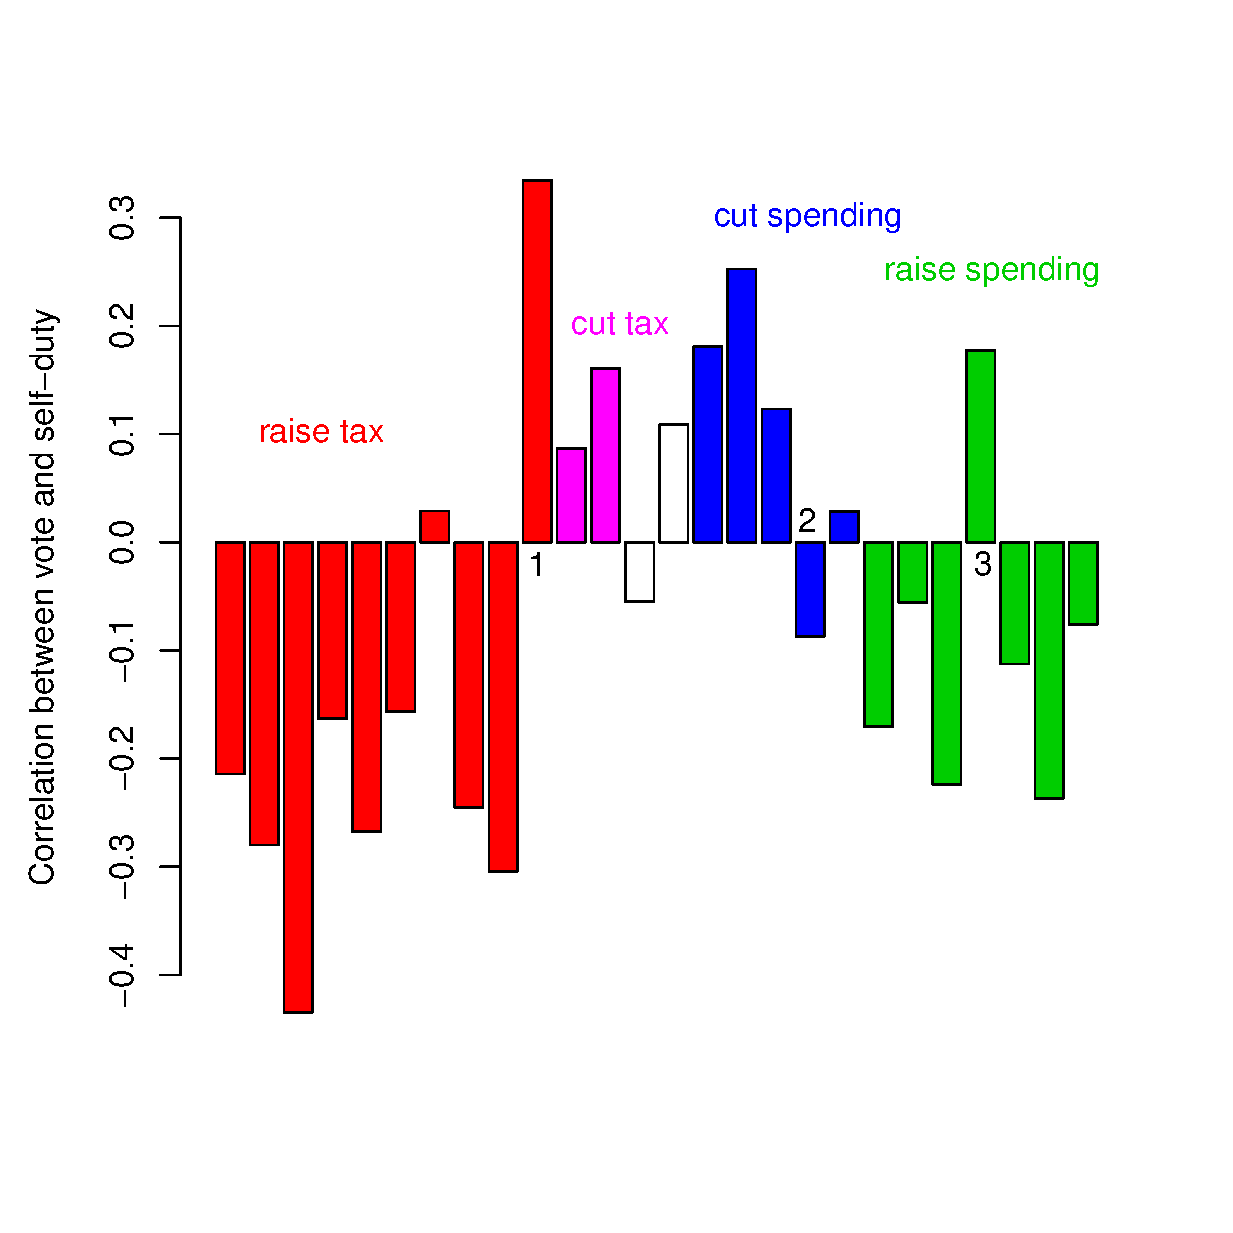
\includegraphics[width=\textwidth]{dut11.eps}
\caption{The caption goes under the figure like this. Note that
  textwidth is the width of the text. But you can use any units,
  e.g., ``3in'' or ``50mm''.}
\end{figure}

\section{Discussion}
It turns out that $E = MC^2$.  Specifically,
\begin{equation}
E = \frac { \sum_{i=1}^n ( M_i C )^2 }{ \alpha + \beta }
\end{equation}
Equation 1 is true.

\subsection{How to write Mathematics}

\LaTeX{} is great at typesetting mathematics. Let $X_1, X_2, \ldots,
X_n$ be a sequence of independent and identically distributed random
variables with $\text{E}[X_i] = \mu$ and $\text{Var}[X_i] = \sigma^2 <
\infty$, and let
\[S_n = \frac{X_1 + X_2 + \cdots + X_n}{n}
      = \frac{1}{n}\sum_{i}^{n} X_i\]
denote their mean. Then as $n$ approaches infinity, the random
variables $\sqrt{n}(S_n - \mu)$ converge in distribution to a normal
$\mathcal{N}(0, \sigma^2)$.

\subsection{How to add Lists}

You can make lists with automatic numbering \dots

\begin{enumerate}
\item Like this,
\item and like this.
\end{enumerate}
\dots or bullet points \dots
\begin{itemize}
\item Like this,
\item and like this.
\end{itemize}

References should be in APA style. Examples are below.

% FOR BIBTEX USERS INSTEAD OF REFERENCES SECTION
%\bibliographystyle{apalike3}
%\bibliography{bibliography.bib}
% OR CAN ALSO INCLUDE THE BBL FILE AFTER THE NEXT LINE, INSTEAD OF THE LAST LINE
\section*{References}

\begin{hangparas}{1em}{1}

  Aarts, H., \& Dijksterhuis, A. (1999).  How often did I do it?
  Experienced ease of retrieval and frequency estimates of past
  behavior.  \textit{Acta Psychologica, 103}(3), 77--89. \url{http://someurl.html}.

  Barberis, N. \& Thaler, R. (2003). A survey of behavioral finance.
  In G. M. Constantinides, M. Harris \& R. Stultz (Eds.),
  \textit{Handbook of the Economics of Finance,} pp.\ 1053--1123.
  Elsevier Science, North Holland, Amsterdam

\vfill % use this for column breaks
\break

Grice, H. P. (1975).  Logic and conversation. In P. Cole \& J.
L. Morgan, (Eds.), \textit{Speech Acts}, pp.\ 41--58. London: Academic
Press. \url{http://dx.doi.org/3.14159--1x}.
\end{hangparas}

\bigskip
\section*{Appendix}

The asterisk means that these divisions are not numbered.

\subsection*{How to write Mathematics}

This section is completely redundant with the text. Do not do
that. This is just an example.

\LaTeX{} is great at typesetting mathematics. Let $X_1, X_2, \ldots, X_n$ be a sequence of independent and identically distributed random variables with $\text{E}[X_i] = \mu$ and $\text{Var}[X_i] = \sigma^2 < \infty$, and let
\[S_n = \frac{X_1 + X_2 + \cdots + X_n}{n}
      = \frac{1}{n}\sum_{i}^{n} X_i\]
denote their mean. Then as $n$ approaches infinity, the random variables $\sqrt{n}(S_n - \mu)$ converge in distribution to a normal $\mathcal{N}(0, \sigma^2)$.


\subsection*{How to create Sections and Subsections}

Use section and subsections to organize your document. Simply use the section and subsection buttons in the toolbar to create them, and we'll handle all the formatting and numbering automatically.

\end{document}
